\documentclass[document.tex]{subfiles}
\begin{document}
\chapter{Experimental Evaluation}
\section{Introduction}
The experiments are complicated by the fact that \textbf{PWPS} is limited to single equations of percentage word problems, and ALGES
can only handle single-equations algebra problem with only addition, subtraction, multiplication and division. Our main experimental result is to find the solution of Percentage word problems.

For experiment our system \textbf{PWPS}, there is two parts. One is Experimental Setup and the other is Dataset. In the following section, I have discussed those in details.
\section{Experimental Setup}
We use the Stanford Dependency Parser in CoreNLP 3.4\cite{32} to obtain syntactic information used for
grounding and feature computation. For the ILP
model, we use CPLEX 12.6.1 (IBM ILOG, 2014)\cite{33}
to generate the top $M = 100$ equation trees with
a maximum stack depth of 10, aborting exploration
upon hitting $10K$ feasible solutions or $30$ seconds.
We use Python’s SymPy package for solving equations for the unknown. For the local and global models,we use Random forest classifier \cite{34,35}(Discussed in Appendix A).
We have used \textbf{Linux (Ubuntu 16.04 LTS)} as our operating system. So, the following process shown only for Linux Environment.
%\subsection{Java Installation}
%For installing Java Compiler, the following command should run from the terminal.
%\begin{center}
%	\begin{lstlisting}
%	sudo apt-get install default-jdk
%	sudo apt-get install default-jre
%	\end{lstlisting}
%\end{center}
%
%\subsection{Python v2.0 and PIP}
%We used \textbf{python 2} as our programming language. For installing Python 2 and Pip, the following command should run from the terminal.
%\begin{center}
%	\begin{lstlisting}
%	sudo apt-get install python2
%	sudo apt-get install pip2
%	\end{lstlisting}
%\end{center}
%
%\subsection{Stanford Dependency Parser CoreNLP 3.4 Server}
%For parser, we have used Stanford Dependency Parser CoreNLP 3.4. This is available at \url{http://nlp.stanford.edu/software/stanford-corenlp-full-2014-06-16.zip}
%
%\subsection{Running Server}
%Following command should run for installing the server essentials and other packages
%\begin{lstlisting}
%sudo pip install pexpect unidecode jsonrpclib 
%git clone https://bitbucket.org/torotoki/corenlp-python.git
%cd corenlp-python
%wget http://nlp.stanford.edu/software/stanford-corenlp-full-2014-08-27.zip
%unzip stanford-corenlp-full-2014-08-27.zip
%\end{lstlisting}
%Then, to launch a server:
%\begin{lstlisting}
%python corenlp/corenlp.py
%\end{lstlisting}
%Optionally, you can specify a host or port:
%\begin{lstlisting}
%python corenlp/corenlp.py -H 0.0.0.0 -p 3456
%\end{lstlisting}
%That will run a public JSON-RPC server on port 3456.
%And you can specify Stanford CoreNLP directory:
%\begin{lstlisting}
%python corenlp/corenlp.py -S stanford-corenlp-full-2014-08-27/
%\end{lstlisting}
%\subsection{PWPS Running}
%To get our code run the following command:
%\begin{lstlisting}
%git clone https://github.com/habibrahmanbd/PWPS
%\end{lstlisting}
%After that, for running our system:
%\begin{lstlisting}
%cd PWPS/
%./PWPS problemset.json
%\end{lstlisting}
%where, \textbf{$problemset.json$} is the dataset.

\section{Dataset Description}
This work deals with percentage word problems that map to single equations with varying length. Every equation may involve multiple math operations including multiplication, division, subtraction, and addition over non-negative rational numbers and one variable. A sample data in JSON format is shown in the Fig. \ref{fig:data} .
\begin{figure}[H]
	\begin{center}
		\begin{lstlisting}
{
	"iIndex": 121,
	"lSolutions": [ 28.0 ],
	"lEquations": [ "x=56.0*(50.0/100.0)" ],
	"sQuestion": " Beth took a math quiz last week. There were 56 problems on the quiz and Beth answered 50% of them correctly. How many problems did Beth get correct? "
}
		\end{lstlisting}
	\end{center}
	\caption{Sample Dataset in JSON Format}
	\label{fig:data}
\end{figure}

We collected a new dataset from \url{http://math-aids.com}, \url{http://ixl.com}, \url{https://www.khanacademy.org} and \url{http://algebra.com}. Dataset statistics is given below in TABLE \ref{tab:datasetstat}.

\begin{table}[H]
	\caption{Dataset Statistics}
	\begin{center}
		\begin{tabular}{|l | r|}
			\hline
			\textbf{Statistics}& \# \\ \hline
			Number of Problems in Dataset& 185 \\
			Number of Sentences in Dataset& 592\\
			Number of Words in Dataset& 5698\\
			Average Sentences per Problem& 3.2\\
			Average Words per Problem& 30.8\\
			\hline
		\end{tabular}
	\end{center}
	\label{tab:datasetstat}
\end{table}

\section{Implementation Procedure} In this section, we have shown the overall procedure with example. We have discussed the theory in chapter 3.

\subsection{Converting Problem Text into Fraction}
The number with ``Percent'' converted to fraction in this section. Fig. \ref{fig:i_conv} shows an example:
\begin{figure}[H]
	\fbox{
		\begin{minipage}{0.96\textwidth}
			Alice has 50 books. She gives her \textbf{0.50 times} books to Bob. How many books Alice have?
		\end{minipage}
	}
	
	\caption{Converted to Fraction and ‘\%’ sign replace by ‘times’ in the problem text}
	\label{fig:i_conv}
\end{figure}

\subsection{Tokenize, Replace, and Grounding}
After tokennize and replacing with keyword, grounded the problem text into several properties. Fig. \ref{fig:i_ground} shows an example of grounding for the problem in \ref{fig:i_conv}.
\begin{figure}[H]
	\fbox{
		\begin{minipage}{0.3\textwidth}
			adjs : None\\
			compound : 0\\
			container : Alice\\
			contains : None\\
			entity : book\\
			idx : 2\\
			location : None\\
			num : 50\\
			origs : 0\\
			role : do\\
			subset : 0\\
			subtypes : []\\
			surface : books\\
			type failure : 0\\
			verbs : has\\
			widx : 4
		\end{minipage}
		
	}
	\fbox{
		\begin{minipage}{0.3\textwidth}
				adjs : None\\
				compound : 0\\
				container : None\\
				contains : None\\
				entity : Alice\\
				idx : 1003\\
				location : None\\
				num : 0.5\\
				origs : 1\\
				role : other\\
				subset : 0\\
				subtypes : []\\
				surface : times\\
				type failure : 0\\
				verbs : give\\
				widx : 5
		\end{minipage}
	}
	\fbox{	
		\begin{minipage}{0.3\textwidth}
			adjs : None\\
			compound : 0\\
			container : Alice\\
			contains : None\\
			entity : book\\
			idx : 2002\\
			location : None\\
			num : x\\
			origs : 2\\
			role : do\\
			subset : 0\\
			subtypes : []\\
			surface : books\\
			type failure : 0\\
			verbs : have\\
			widx : 3
		\end{minipage}
	}
	\caption{Grounded Qsets from Fig. \ref{fig:i_conv}}
	\label{fig:i_ground}
\end{figure}
\subsection{Integer Linear Programming}
ALGES uses \textbf{Integer Linear Programming (ILP)} to generate equation trees from the base Qsets. These equations are then used for learning and inferencing the system PWPS and selects best \textit{M} candidate equations for a given problem text, \textit{p}.

For problem text, \textit{p} and \textit{n} base Qsets, PWPS builds \textit{ILP(P)} over the space of postfix equations $ E = e_1, e_2,...,e_L $ of length L  and k numeric constants, $k'  = n – k$ unknowns, \textit{r} binary operators and \textit{q} \textit{“types”} of Qsets like ALGES.

\begin{figure}[H]
	\begin{center}
	\fbox{
		\begin{minipage}{0.3\textwidth}
			quantities : 50 0.5 x\\
			types : "book" "Alice" "book"\\
			operators : + - * / =\\
			n : 5\\
			answer : 25.0
		\end{minipage}
	}
	\end{center}
	\caption{Preprocessing before ILP}
	\label{fig:i_Pre_ILP}
\end{figure}
Before generating equation tree, ILP uses the properties in \ref{fig:i_Pre_ILP}. After that, it passes through the ILP to generate the equation tree. Fig. \ref{fig:i_ILP} shows the tree generated by ILP:
\begin{landscape}
\begin{figure}
	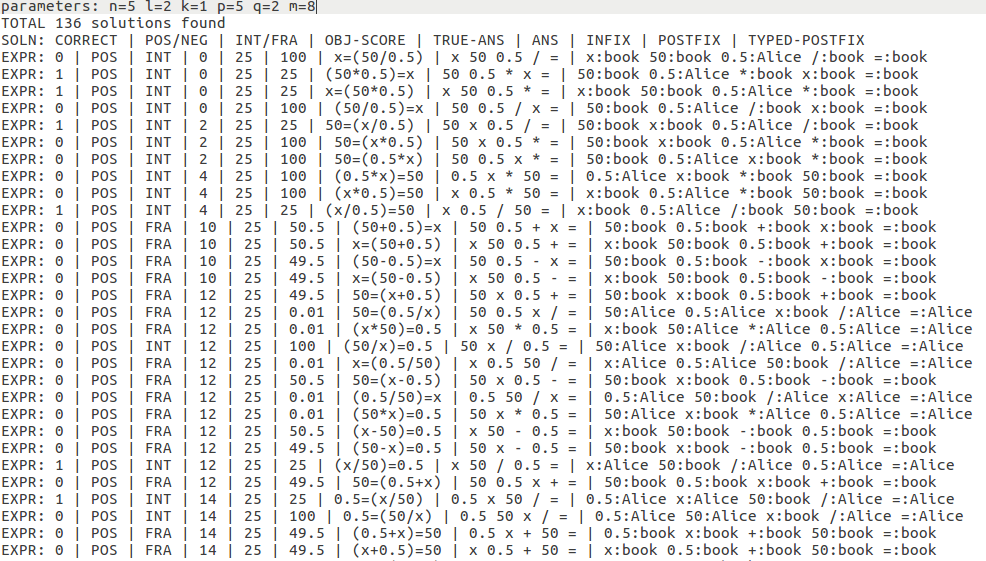
\includegraphics[scale=0.68]{imgs/ILP_tree.png}
	\caption{Tree generation by ILP}
	\label{fig:i_ILP}
\end{figure}
\end{landscape}
\begin{landscape}
\subsection{Local Qset Relationship Model Features}
 Given the richness of the textual possibilities for indicating a math operation, the features are designed over semantic and intertextual relationships between Qsets, as well as domain-specific lexical features. Fig. \ref{fig:i_Local} shows the feature extracted: 

	\begin{figure}[H]
		\includegraphics[scale=0.520]{imgs/"Local Model Features".png}
		\caption{Features extracted for local model}
		\label{fig:i_Local}
	\end{figure}
	\subsection{Global equation Model Features}
	Features $f_{global}$ are explained in Table \ref{tab:landg}. They include the number of violated soft constraints in the
	ILP, the probabilities of the left and right subtrees of
	the root as provided by the local model, and global
	lexical features. Features extracted shown in Fig. \ref{fig:i_global}. 
	
	\begin{figure}[H]
		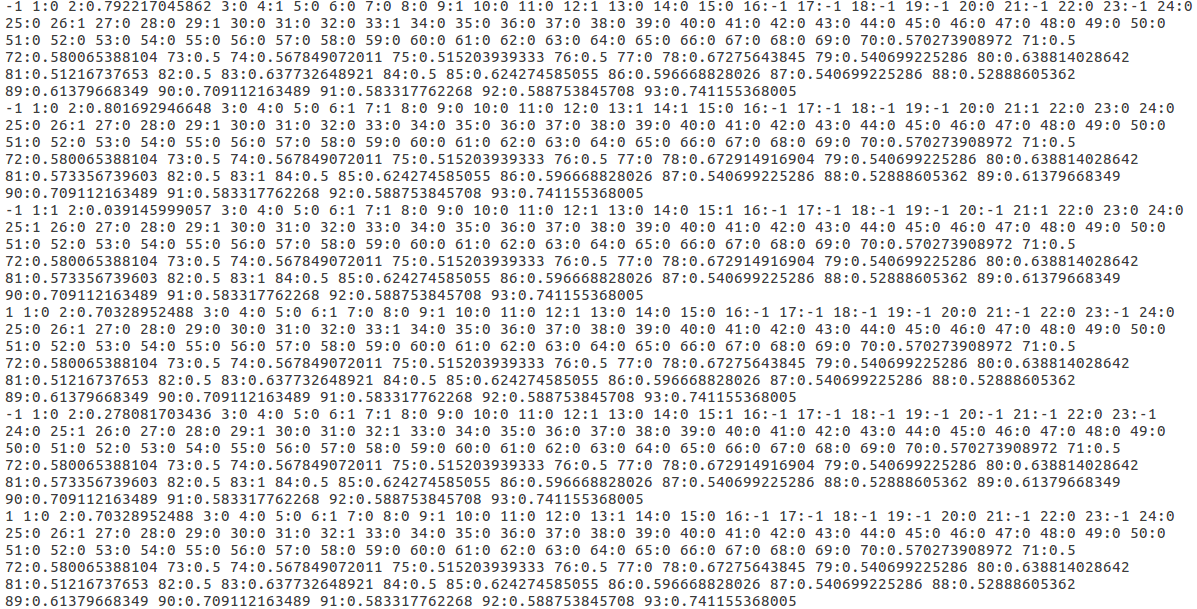
\includegraphics[scale=0.500]{imgs/global_features.png}
		\caption{Feature Extracted for global model}
		\label{fig:i_global}
	\end{figure}
\end{landscape}
\section{Conclusion} In this chapter, we have shown the dataset description, environmental setup and implementation procedure with an example. The experiments are complicated by the fact that \textbf{PWPS} is limited to single equations of percentage word problems, and ALGES can only handle single-equations algebra problem with only addition, subtraction, multiplication and division. Our main experimental result is to find the solution of Percentage word problems. In the next chapter, we have showed the result and performance analysis.
\end{document}
